% !TEX TS-program = pdflatex
% !TEX encoding = UTF-8 Unicode

% This is a simple template for a LaTeX document using the "article" class.
% See "book", "report", "letter" for other types of document.

\documentclass[11pt]{article} % use larger type; default would be 10pt

\usepackage[utf8]{inputenc} % set input encoding (not needed with XeLaTeX)

%%% Examples of Article customizations
% These packages are optional, depending whether you want the features they provide.
% See the LaTeX Companion or other references for full information.

%%% PAGE DIMENSIONS
\usepackage{geometry} % to change the page dimensions
\geometry{a4paper} % or letterpaper (US) or a5paper or....
% \geometry{margin=2in} % for example, change the margins to 2 inches all round
% \geometry{landscape} % set up the page for landscape
%   read geometry.pdf for detailed page layout information

\usepackage{graphicx} % support the \includegraphics command and options

% \usepackage[parfill]{parskip} % Activate to begin paragraphs with an empty line rather than an indent

%%% PACKAGES
\usepackage{booktabs} % for much better looking tables
\usepackage{array} % for better arrays (eg matrices) in maths
\usepackage{paralist} % very flexible & customisable lists (eg. enumerate/itemize, etc.)
\usepackage{verbatim} % adds environment for commenting out blocks of text & for better verbatim
\usepackage{subfig} % make it possible to include more than one captioned figure/table in a single float
\usepackage{graphicx}
\usepackage{float}
\usepackage{cite} 
\usepackage{url}
\usepackage{amsmath}
\usepackage{hyperref}

% These packages are all incorporated in the memoir class to one degree or another...

%%% HEADERS & FOOTERS
\usepackage{fancyhdr} % This should be set AFTER setting up the page geometry
\pagestyle{fancy} % options: empty , plain , fancy
\renewcommand{\headrulewidth}{0pt} % customise the layout...
\lhead{}\chead{}\rhead{}
\lfoot{}\cfoot{\thepage}\rfoot{}

%%% SECTION TITLE APPEARANCE
\usepackage{sectsty}
\allsectionsfont{\sffamily\mdseries\upshape} % (See the fntguide.pdf for font help)
% (This matches ConTeXt defaults)

%%% ToC (table of contents) APPEARANCE
\usepackage[nottoc,notlof,notlot]{tocbibind} % Put the bibliography in the ToC
\usepackage[titles,subfigure]{tocloft} % Alter the style of the Table of Contents
\renewcommand{\cftsecfont}{\rmfamily\mdseries\upshape}
\renewcommand{\cftsecpagefont}{\rmfamily\mdseries\upshape} % No bold!

%%% END Article customizations

%%% The "real" document content comes below...

\title{ Automated approaches to assess the similarity of open source projects. }

\author{Rubei Riccardo}
%\date{} % Activate to display a given date or no date (if empty),
         % otherwise the current date is printed 

\begin{document}
\maketitle
\newpage
\tableofcontents
\newpage




%Introduction
%% Mention CROSSMINER THe work has been done in that context...

%Mearuring the Similarty of SOftwre Systems
% %You can use some of the content from D6.2. Hopefully, CROSSSim can be included in this section as existing work (saying that it has been developed in the context of CROSSMINER

%Detailed description of the CLAN implementation

%Detailed description of the MUDABlue implementation

% Comparison CROSSSIM,CLAN and MUDABlue, RepoPal
%% Conduct evaluatin on the dataset f 580 Github projects


% Conclusion and Future Work






		\section{Introduction}
		\label{sec:Introduction}
		\subsection{Summary}
Open source software (OSS) repositories contain a large amount of data that has been accumulated along the software development process. Not only source code but also metadata available from different related sources, e.g. communication channels, bug tracking systems, is beneficial to the development process once it is properly mined. Research has been performed to understand and predict software evolution, exploiting the rich metadata available at OSS repositories. This allows for the reduction of effort in knowledge acquisition and quality gain. Developers can leverage the underlying knowledge if they are equipped with suitable tools. For instance, it is possible to empower IDEs by means of tools that continuously monitor the developer's activities and contexts in order to activate dedicated recommendation engines \cite{Ponzanelli:2014:MST:2597073.2597077}. 

%To aim for software quality, for developers it is necessary to understand how similar, mature projects are developed.   it is necessary

To aim for software quality, developers normally build their project by learning from mature OSS projects having comparable functionalities. To this end, the ability to search for similar software projects with respect to different criteria such as functionalities and dependencies plays an important role in the development process. Two projects are deemed to be similar if they implement some features being described by the same abstraction, even though they may contain various functionalities for different domains \cite{McMillan:2012:DSS:2337223.2337267}. Understanding the similarities between open source software projects allows for reusing of source code and prototyping, or choosing alternative implementations \cite{Schafer:2007:CFR:1768197.1768208},\cite{10.1109/SANER.2017.7884605}, thereby improving software quality. Meanwhile measuring the similarities between developers and software projects is a critical phase for most types of recommender systems \cite{DBLP:conf/rweb/NoiaO15},\cite{Sarwar:2001:ICF:371920.372071}. Similarities are used as a base by both content-based and collaborative-filtering recommender systems to choose the most suitable and meaningful items for a given item \cite{Schafer:2007:CFR:1768197.1768208}. Failing to compute precise similarities means concurrently adding a decline in the overall performance of these systems. Nevertheless, measuring similarities between software systems has been considered as a daunting task \cite{Chen:2015:SFD:2684822.2685305},\cite{McMillan:2012:DSS:2337223.2337267}. Furthermore, considering the miscellaneousness of artifacts in open source software repositories, similarity computation becomes more complicated as many artifacts and several cross relationships prevail.

In recent years, considerable effort has been made to provide automated assistance to developers in navigating large information spaces and giving recommendations. Though remarkable progress can be seen in this field, there is still room for improvement. To the best of our knowledge, most of the existing approaches consider the constituent components of the OSS ecosystem separately, without paying much attention to their mutual connections. There is a lack of a proper scheme that facilitates a unified consideration of various OSS artifacts and recommendations. 

CROSSMINER\footnote{\url{https://www.crossminer.org}} is a research project funded by the EU Horizon 2020 Research and Innovation Programme, aiming at supporting the development of complex software systems by \textit{i)} enabling monitoring, in-depth analysis and evidence-based selection of open source components, and \textit{ii)} facilitating knowledge extraction from large OSS repositories \cite{10.1007/978-3-319-74730-9_33}. In the context of the project, we work towards an advanced Eclipse-based IDE providing intelligent recommendations that go far beyond the current \emph{code completion-oriented} practice. Among others, an indispensable functionality is to find a set of similar OSS projects to a given project with respect to different criteria, such as external dependencies, application domain, or API usage \cite{NDRDSEAA2018},\cite{DBLP:conf/iir/NDD013}.

The purpose of this thesis is the implementation of two approaches, MUDABlue and Clan, with the aim of compare the results of new tool by CROSSMINER development team (CrossSim). CROSSSIM (Cross Project Relationships for Computing Open Source Software Similarity), is an approach that makes use of graphs for rep-resenting different kinds of relationships in the OSS ecosystem. In particular, with the adoption of the graph representation, we are able to transform the relationships among non-human artifacts, e.g. API utilizations, source code, interactions, and humans, e.g. developers into a mathematically computable format, i.e. one that
facilitates various types of computation techniques. Naturally this kind of approaches has to be evaluated, and confronted with others similar tools. My work helps addressing this challenge providing these two tools and evaluating all the results to show how nice is CrossSim.
		\clearpage

		\section{Crossminer Project}
		\label{sec:Crossminer Project}
		\subsection{CROSSMINER}

\subsubsection{Open Source Software Challenges}
Open-source software (OSS) is computer software available in source code form, for which the source code and certain other rights are provided under a license that permits users to study, change, and improve the software for free. A report by Standish Group states that adoption of open-source software models has resulted in savings of about 58 billion per year to consumers. Unlike commercial software which is typically developed within the context of a particular organisation with a well-established business plan and commitment to the maintenance, documentation and support of the software, OSS is very often developed in a public, collaborative, and loosely-coordinated manner. This has several implications to the level of quality of different OSS software as well as to the level of support that different OSS communities provide to users of the software they produce.
There are several high-quality and mature OSS projects that deliver stable and well-documented products. Such projects typically also foster a vibrant expert and user community, which provides remarkable levels of support both in answering user questions and in repairing reported defects in the provided software. However, there are also many OSS projects that are dysfunctional in one or more of the following ways:
\begin{itemize}
	\item The development team behind the OSS project invests little time on its development, maintenance and support.
	\item The development of the project has been altogether discontinued due to lack of commitment or motivation.
	\item The documentation of the produced software is limited and/or of poor quality
	\item The source code contains little or low-quality comments which make studying and maintaining it challenging
	\item The community around the project is limited, and questions asked by users receive late/no response and identified defects either get repaired very slowly or are altogether ignored
\end{itemize}
Consequently, developing new software systems by reusing existing open source components raises relevant challenges related to the following activities:
\begin{itemize}
	\item Searching for candidate components.
	\item Evaluating a set of retrieved candidate components to find the most suitable one.
	\item Adapting the selected components to fit the specific requirements.
\end{itemize}


\subsubsection{Selecting Open Source Components}
Deciding whether open source software (OSS) meets the required standards for adoption in terms of quality, maturity, activity of development and user support is not a straightforward process. It involves exploring various sources of information including:
\begin{itemize}
\item Its source code repositories to identify how actively the code is developed, how well the code is commented, whether there are unit tests etc.

\item Communication channels such as newsgroups, forums and mailing lists to identify whether user questions are answered in a timely and satisfactory manner, to estimate the number of experts and users of the software

\item Its bug tracking system to identify whether the software has many open bugs and at which rate bugs are fixed, and

\item Other relevant metadata such as the number of downloads, the license(s) under which it is made available, its release history etc.
\end{itemize}
Dependence on an OSS project can thus either be a blessing or a curse. The ability to accurately assess the risks and benefits of adopting particular OSS projects is essential to the software community at large - especially open source software frameworks and platforms and highly specialised essential utility packages, which can make a depending product or service unexpectedly incur insurmountable technical difficulties when the OSS projects suddenly reach end-of-life.

\subsubsection{Project Technologies}
The overarching aim of CROSSMINER is to deliver an integrated open-source platform that will support the development of complex software systems by (1) enabling monitoring, in-depth analysis and evidence-based selection of open source components, and (2) facilitating knowledge extraction from large open-source software repositories. The six main scientific and technology objectives for the project are the following:
\begin{itemize}
\item Development of source code analysis tools to extract and store actionable knowledge from the source code of a collection of open-source projects

\item Development of natural language analysis tools to extract quality metrics related to the communication channels, and bug tracking systems of OSS projects by using Natural Language Processing and text mining techniques

\item Development of system configuration analysis tools to gather and analyse system configuration artefacts and data to provide an integrated DevOps-level view of a considered open source project

\item Development of workflow-based knowledge extractors that simplify the development of bespoke analysis and knowledge extraction tools shielding engineers from technological issues to concentrate on core analysis tasks

\item Development of cross-project relationship analysis tools to manage a wider range of open source project relationships, such as dependencies and conflicts, based on user-defined similarity measures underpinning the automated creation of project clusters.

\item Development of advanced integrated development environments that will allow developers to adopt the CROSSMINER knowledge base and analysis tools directly from the development environment, while providing alerts, recommendations, and user feedback which will help developers to improve their productivity.
\end{itemize}
The outcomes of the different CROSSMINER analysis tools will contribute to the definition of a knowledge base supporting multidimensional classifications of projects and disclosing a number of applications such as automated identification of complementary and competing projects, project incompatibilities and prediction of the future of given projects based on the evolution of other projects having similar characteristics in the past.
		\clearpage

		\section{The Similarity Problem}
		\label{sec:Similarity}
		\subsection{Overview}

Text similarity measures play an increasingly important role in text related research and applications in tasks such as information retrieval, text classification, document clustering, topic detection, topic tracking, questions generation, question answering, essay scoring, short answer scoring, machine translation, text summarization and others. Finding similarity between words is a fundamental part of text similarity which is then used as a primary stage for sentence, paragraph and document similarities. There two way in which words can be similar each other, lexically if they share sequences of characters similar and  semantically if are used in the same context, used in the same way and so on. 

%%%%%%%%%%%%%%%%%%%%%%%%%%%%%%%%%%%%%%%%%%%%%%%%%%%%%%%%%%

\subsection{String-Based}

The world of lexical similarity con be divided in two categories: character-based and word-based.
To better understand what character-based means, here one of the most well known technique: Levenshtein distance.
\subsubsection{ Levenshtein distance}
 Levenshtein distance defines distance between two strings by counting the minimum number of operations needed to transform one string into the other, where an operation is defined as an insertion, deletion, or substitution of a single character, or a transposition of two adjacent characters.

This is an example:

\begin{itemize}
    \item kitten to sitten (substitution of "s" for "k").
    \item sitten to sittin (substitution of "i" for "e").
    \item sittin to sitting (insertion of "g" at the end).
\end{itemize}

Moving to the word-based,  the word or string similarity measures operate on string sequences and character composition. A string metric is a metric that measures similarity or dissimilarity (distance) between two text strings for approximate string matching or comparison.

\newpage
\subsubsection{Cosine Similarity}

Cosine similarity is a metric used to compute similarity between two objects using their feature vectors \cite{tversky1977features}. An object is characterized as a vector, and for a pair of vectors $\vec{\alpha}=(\alpha_{1},\alpha_{2},..,\alpha_{n})$ and $\vec{\beta}=(\beta_{1},\beta_{2},..,\beta_{n})$ there is an angle between them. Intuitively, the cosine similarity metric measures the similarity as the cosine of the corresponding angle between the two vectors and it is computed using the inner product as follows. 

\begin{equation} \label{eqn:Cosine}
CosineSim(\vec{\alpha},\vec{\beta}) = \frac{\sum_{i=1}^{n}\alpha_{i}\cdot \beta_{i}}{\sqrt{\sum_{i=1}^{n}(\alpha_{i})^{2} }\cdot \sqrt{\sum_{i=1}^{n}(\beta_{i})^{2}}}
\end{equation}

Figure \ref{fig:Cosine} illustrates the cosine similarity between two vectors $\vec{\alpha}$ and $\vec{\beta}$ in a three-dimension space. This can be thought as the similarity between two documents with three terms $t=(t_{1},t_{2},t_{3})$.

\begin{figure}[h!]
	\centering
	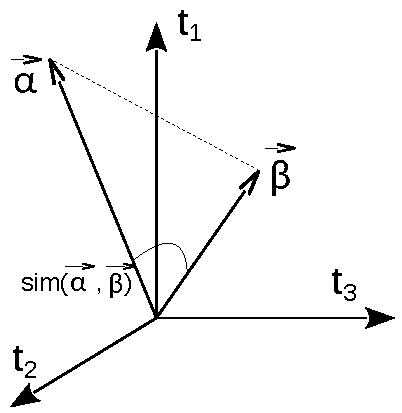
\includegraphics[width=0.25\textwidth]{images/Cosine.pdf}
	\caption{Cosine similarity between two feature vectors $\vec{\alpha}$ and $\vec{\beta}$}
	\label{fig:Cosine}
\end{figure}

Cosine similarity has been popularly adopted in many applications that are related to similarity measurement in various domains \cite{Huang:2012:LCD:2343876.2343884},\cite{Islam:2008:STS:1376815.1376819},\cite{Linden:2003:ARI:642462.642471},\cite{conf:iscis:MadylovaO09},\cite{Mihalcea:2006:CKM:1597538.1597662}. Among the similarity metrics being recalled in this deliverable, the prevalence of Cosine Similarity is obvious as it is utilized in almost all of them as follows: \textit{MUDABlue} \cite{10.1109/APSEC.2004.69}, \textit{CLAN} \cite{McMillan:2012:DSS:2337223.2337267}, \textit{CLANdroid} \cite{10.1109ICPC.2016.7503721}, \textit{LibRec} \cite{6671293}, \textit{SimApp} \cite{Chen:2015:SFD:2684822.2685305}, \textit{WuKong} \cite{Wang:2015:WSA:2771783.2771795}, \textit{TagSim} \cite{Lo:2012:DSA:2473496.2473616}, and \textit{RepoPal} \cite{10.1109/SANER.2017.7884605}.\\

This is an example of how the cosine similarity can be done  between two sentences.
These are the two string that we want to compare to see how much they are related each other.

\begin{itemize}
\item Julie loves me more than Linda loves me.
\item Jane likes me more than Julie loves me.
\end{itemize}
\newpage
From the strings is possible to count the occurrencies of each term, putting everything in a matrix.
\begin{figure}
	\begin{equation} \nonumber
	\bordermatrix{~ & string 1 & string 2 \cr	
		me 		& 2 & 2  \cr 
		Jane		& 0 & 1  \cr  
		Julia		& 1 & 1  \cr
		Linda 		& 1 & 0  \cr 
		likes		& 0 & 1  \cr
		loves		& 2 & 1  \cr
		more		& 1 & 1  \cr
		than		& 1 & 1  \cr	}
	\end{equation}
	\caption{The occurrencies.}
	\label{fig:TDM}
\end{figure}

Since in this kind of evaluation is not important the meaning or where the words are, is possibile to create the related vectore in order to compute the similarity.\\

	\begin{equation} \nonumber
	String1 = [2, 0, 1, 1, 0, 2, 1, 1]
	\end{equation}

	\begin{equation} \nonumber
	String2 = [2, 1, 1, 0, 1, 1, 1, 1]
	\end{equation}

Applying the cosine similarity formula this is the outcome:

\begin{equation} \label{eqn:Cosine}
CosineSim(\vec{\alpha},\vec{\beta}) = \frac{9}{\sqrt{12}\cdot \sqrt{10}} = 0.822
\end{equation}
This means that these strings are close each other 0.822, in a range bewteen 0.0 and 1.0.

%%%%%%%%%%%%%%%%%%%%%%%%%%%%%%%%%%%%%%%%%%%%%%%%%%%%%%%%%%  
\subsection{Corpus-Based}
\subsubsection{Term-Document Matrix}
 In Natural Language Processing \cite{Collobert:2011:NLP:1953048.2078186}, a term-document matrix (TDM) is used to represent the relationships between words and documents \cite{Turney:2010:FMV:1861751.1861756}. In a TDM, each row corresponds to a document and each column corresponds to a term. A cell in the TDM represents the weight of a term in a document. The most common weighting scheme used in document retrieval is the \emph{term frequency-inverse document frequency (tf-idf)} function \cite{Reed:2006:TNT:1193211.1193734}. If we consider a set of $n$ documents $D=(d_{1},d_{2},..,d_{n})$ and a set of terms $t=(t_{1},t_{2},..,t_{r})$ then the representation of a document $d \in D $ is vector $\vec{\delta}=(w_{1}^{d},w_{2}^{d},..,w_{r}^{d})$, where the weight $w_{k}^{d}$ of term $k$ in document $d$ is computed using the {\em tf-idf} function \cite{Ramos1999}:

\begin{equation} \label{tfidf} %\nonumber 
w_{k}^{d} =tf\cdot idf(k,d,D)= f_{k}^{d}\cdot log\frac{n}{\left | \left \{ d\in D: t_{k} \in d \right \} \right |} 
\end{equation}

where $f_{k}^{d}$ is the frequency of term $t_{k}$ in document $d$.

Another common weighting scheme uses only the frequency of terms in documents for cells in TDM, i.e. the number of occurrence of a term in a document, instead of {\em tf-idf}. As an example, we consider a set of three simple documents $D=(d_{1},d_{2},d_{3})$ as follows:

\begin{itemize}
	\item[+] $d_{1}$: \emph{She is nice.}
	\item[+] $d_{2}$: \emph{Today is nice.}
	\item[+] $d_{3}$: \emph{Nice is a nice city.}
\end{itemize}

\begin{figure}[h!]
	\begin{equation} \nonumber
	\bordermatrix{~ & she & is & today & a & nice & city \cr	
		d_{1} 		& 1 & 1 & 0 & 0 & 1 & 0 \cr 
		d_{2} 		& 0 & 1 & 1 & 0 & 1 & 0 \cr  
		d_{3} 		& 0 & 1 & 0 & 1 & 2 & 1 \cr }
	\end{equation}
	\caption{An example of a term-document matrix}
	\label{fig:TDM}
\end{figure}

The set of terms $t$ consists of $6$ elements, i.e. $t=(she$, $is$, $today$, $a$, $nice$, $city)$ and the corresponding term-document matrix for $D$ is depicted in Figure \ref{fig:TDM}.

TDM has been exploited to characterize software systems and finally to compute similarities between them \cite{10.1109/APSEC.2004.69},\cite{10.1109ICPC.2016.7503721},\cite{McMillan:2012:DSS:2337223.2337267}. In a TDM for software systems, each row represents a package, an API call or a function and each column represents a software system. A cell in the matrix is the number of occurrence of a package/an API/function in each corresponding software system. A TDM for software systems has a similar form to the matrix shown in Figure \ref{fig:TDM} where documents are replaced by software systems and terms are replaced by API calls.

\subsubsection{Latent Semantic Analysis}

The problem with the term-document matrix is that the intrinsic relationships among different terms of a document cannot fully be captured. Furthermore, same words can be used to explain different requirements or the other way around, the same requirements can be described using different words \cite{10.1109/APSEC.2004.69}. Latent Semantic Analysis (LSA), also known as Latent Semantic Indexing (LSI), has been proposed to overcome these problems \cite{Landauer1998}. The technique exploits a mathematical model that can infer latent semantic relationships to compute similarity. LSA represents the contextual usage meaning of words by statistical computations applied to a large corpus of text. It then generates a representation that captures the similarity of words and text passages. To perform LSA on a text, a term-document matrix is created to characterize the text. Afterwards, Singular Value Decomposition (SVD) - a matrix decomposition technique - is used in combination with LSA to reduce matrix dimensionality \cite{kb2005}. SVD takes a highly variable set of data entries as input and transforms to a lower dimensional space but reveals the substructure of the original data. Essentially, it decomposes a rectangular matrix into the product of three other matrices as given below\cite{kb2005}:

\begin{equation}
A_{mn}=U_{mm}S_{mn}V_{mn}^{T}
\end{equation}

in which

\begin{itemize}
	\item $U_{mm}$: Orthogonal matrix.
	\item $S_{mn}$: Diagonal matrix.
	\item $V_{mn}^{T}$: The transpose of an orthogonal matrix.
	\item $X$: Low Rank matrix.
\end{itemize}


$U_{mm}$ describes the original row entities as vectors of derived orthogonal factor values. $S_{mn}$ represents the original column entities in the same way, and $V_{mn}$ is a diagonal matrix containing scaling values. With the application of LSA it is possible to find the most relevant features and remove the least important ones by means of the reduced matrix $U_{mm}$. As a result, an equivalence of $A_{mm}$ can be constructed using the most relevant features. LSA helps reveal the latent relationship among words as well as among passages which cannot be guaranteed by a simple term-document matrix. The similarity measurement by LSA reflects adequately human perception of similarity and association among texts. Using LSA, similarities among documents are measured as the cosine of the angle between their row vectors (see Sec. \ref{sec:cosine}). LSA has been applied in \cite{10.1109/APSEC.2004.69},\cite{10.1109ICPC.2016.7503721},\cite{McMillan:2012:DSS:2337223.2337267} to compute similarities of software systems. The main disadvantage of LSA is that it is computational expensive when a large amount of information is analyzed.

\newpage

An example.
Image that these are a set of document to be analyzed and we want to apply the procedure stated before.
\begin{itemize}
	\item doc1: Human machine interface for ABC computer applications
	\item doc2: A survey of user opinion of computer system response time
	\item doc3: The EPS user interface management system
	\item doc4: System and human system engineering testing of EPS
	\item doc5: Relation of user perceived response time to error measurement
	\item doc6: The generation of random, binary, ordered trees
	\item doc7: The intersection graph of paths in trees
	\item doc8: Graph minors IV: Widths of trees and well-quasi-ordering
	\item doc9: Graph minors: A survey
\end{itemize}

\begin{figure}[h!]
	\begin{equation} \nonumber
	\bordermatrix{~ & doc1 & doc2 & doc3 & doc4 & doc5 & doc6 & doc7 & doc8 & doc9 \cr	
		human	& 1 & 0 & 0 & 1 & 0 & 0 & 0 & 0 & 0 \cr
		interface	& 1 & 0 & 1 & 0 & 0 & 0 & 0 & 0 & 0 \cr
		computer	& 1 & 1 & 0 & 0 & 0 & 0 & 0 & 0 & 0 \cr    
		user 		& 0 & 1 & 1 & 0 & 2 & 0 & 0 & 0 & 0 \cr
		system 	& 0 & 1 & 1 & 2 & 0 & 0 & 0 & 0 & 0 \cr
		response	& 0 & 1 & 0 & 0 & 1 & 0 & 0 & 0 & 0 \cr
		time 		& 0 & 0 & 1 & 1 & 0 & 0 & 0 & 0 & 0 \cr
		EPS 		& 0 & 1 & 0 & 0 & 0 & 0 & 0 & 0 & 1 \cr
		survey	& 0 & 0 & 0 & 0 & 0 & 1 & 1 & 1 & 0 \cr
		trees 		& 0 & 0 & 0 & 0 & 0 & 0 & 1 & 1 & 1 \cr
		graph 		& 0 & 0 & 0 & 0 & 0 & 0 & 0 & 1 & 1 \cr
		minors		& 1 & 1 & 0 & 0 & 1 & 0 & 1 & 1 & 0 \cr	  }
	\end{equation}
	\caption{Term-Document matrix related to the example.}
	\label{fig:TDM}
\end{figure}

\begin{figure}[h!]
	\begin{equation} \nonumber
	\bordermatrix{ ~ \cr
		& 0.22 & -0.11 & 0.29 & -0.41 & -0.11 & -0.34 & 0.52 & -0.06 & -0.41 \cr
		& 0.20 & -0.07 & 0.14 & -0.55 & 0.28 & 0.50 & -0.07 & -0.01 & -0.11 \cr
		& 0.24 & 0.04 & -0.16 & -0.59 & -0.11 & -0.25 & -0.30 & 0.06 & 0.49 \cr
		& 0.40 & 0.06 & -0.34 & 0.10 & 0.33 & 0.38 & 0.00 & 0.00 & 0.01 \cr
		& 0.64 & -0.17 & 0.36 & 0.33 & -0.16 & -0.21 & -0.17 & 0.03 & 0.27 \cr
		& 0.27 & 0.11 & -0.43 & 0.07 & 0.08 & -0.17 & 0.28 & -0.02 & -0.05 \cr
		& 0.27 & 0.11 & -0.43 & 0.07 & 0.08 & -0.17 & 0.28 & -0.02 & -0.05 \cr
		& 0.30 & -0.14 & 0.33 & 0.19 & 0.11 & 0.27 & 0.03 & -0.02 & -0.17 \cr
		& 0.21 & 0.27 & -0.18 & -0.03 & -0.54 & 0.08 & -0.47 & -0.04 & -0.58 \cr
		& 0.01 & 0.49 & 0.23 & 0.03 & 0.59 & -0.39 & -0.29 & 0.25 & -0.23 \cr
		& 0.04 & 0.62 & 0.22 & 0.00 & -0.07 & 0.11 & 0.16 & -0.68 & 0.23 \cr
		& 0.03 & 0.45 & 0.14 & -0.01 & -0.30 & 0.28 & 0.34 & 0.68 & 0.18 \cr	  }
	\end{equation}
	\caption{$U_{mm}$x}
	\label{fig:TDM}
\end{figure}

\begin{figure}[h!]
	\begin{equation} \nonumber
	\bordermatrix{~  \cr	
		& 3.34 & 0 & 0 & 0 & 0 & 0 & 0 & 0 & 0 \cr
		& 0 & 2.54 & 0 & 0 & 0 & 0 & 0 & 0 & 0 \cr
		& 0 & 0 & 2.35 & 0 & 0 & 0 & 0 & 0 & 0 \cr
		& 0 & 0 & 0 & 1.64 & 0 & 0 & 0 & 0 & 0 \cr
		& 0 & 0 & 0 & 0 & 1.50 & 0 & 0 & 0 & 0 \cr
		& 0 & 0 & 0 & 0 & 0 & 1.31 & 0 & 0 & 0 \cr
		& 0 & 0 & 0 & 0 & 0 & 0 & 0.85 & 0 & 0 \cr
		& 0 & 0 & 0 & 0 & 0 & 0 & 0 & 0.56 & 0 \cr
		& 0 & 0 & 0 & 0 & 0 & 0 & 0 & 0 & 0.36 \cr
	  }
	\end{equation}
	\caption{ $S_{mn}$}
	\label{fig:TDM}
\end{figure}

\clearpage
\begin{figure}[h!]
	\begin{equation} \nonumber
	\bordermatrix{~  \cr	
		& 0.20 & 0.61 & 0.46 & 0.54 & 0.28 & 0.00 & 0.01 & 0.02 & 0.08 \cr
		& -0.06 & 0.17 & -0.13 & -0.23 & 0.11 & 0.19 & 0.44 & 0.62 & 0.53 \cr
		& 0.11 & -0.50 & 0.21 & 0.57 & -0.51 & 0.10 & 0.19 & 0.25 & 0.08 \cr
		& -0.95 & -0.03 & 0.04 & 0.27 & 0.15 & 0.02 & 0.02 & 0.01 & -0.03 \cr
		& 0.05 & -0.21 & 0.38 & -0.21 & 0.33 & 0.39 & 0.35 & 0.15 & -0.60 \cr
		& -0.08 & -0.26 & 0.72 & -0.37 & 0.03 & -0.30 & -0.21 & 0.00 & 0.36 \cr
		& 0.18 & -0.43 & -0.24 & 0.26 & 0.67 & -0.34 & -0.15 & 0.25 & 0.04 \cr
		& -0.01 & 0.05 & 0.01 & -0.02 & -0.06 & 0.45 & -0.76 & 0.45 & -0.07 \cr
		& -0.06 & 0.24 & 0.02 & -0.08 & -0.26 & -0.62 & 0.02 & 0.52 & -0.45 \cr	 
 }
	\end{equation}
	\caption{$V_{mn}^{T}$}
	\label{fig:TDM}
\end{figure}
The following image depict the result of the decomposition with a rank of 2.
\begin{table}[h!]
	\begin{equation} \nonumber
	\bordermatrix{~ & doc1 & doc2 & doc3 & doc4 & doc5 & doc6 & doc7 & doc8 & doc9 \cr	
		human 	& 0.16 & 0.40 & 0.38 & 0.47 & 0.18 & -0.05 & -0.12 & -0.16 & -0.09 \cr
		interface 	& 0.14 & 0.37 & 0.33 & 0.40 & 0.16 & -0.03 & -0.07 & -0.10 & -0.04 \cr
		computer	& 0.15 & 0.51 & 0.36 & 0.41 & 0.24 & 0.02 & 0.06 & 0.09 & 0.12 \cr
		user 		& 0.26 & 0.84 & 0.61 & 0.70 & 0.39 & 0.03 & 0.08 & 0.12 & 0.19 \cr
		system 	& 0.45 & 1.23 & 1.05 & 1.27 & 0.56 & -0.07 & -0.15 & -0.21 & -0.05 \cr
		response 	& 0.16 & 0.58 & 0.38 & 0.42 & 0.28 & 0.06 & 0.13 & 0.19 & 0.22 \cr
		time 		& 0.16 & 0.58 & 0.38 & 0.42 & 0.28 & 0.06 & 0.13 & 0.19 & 0.22 \cr
		EPS 	 	& 0.22 & 0.55 & 0.51 & 0.63 & 0.24 & -0.07 & -0.14 & -0.20 & -0.11 \cr 
		survey 	& 0.10 & 0.53 & 0.23 & 0.21 & 0.27 & 0.14 & 0.31 & 0.44 & 0.42 \cr
		trees 		& -0.06 & 0.23 & -0.14 & -0.27 & 0.14 & 0.24 & 0.55 & 0.77 & 0.66 \cr
		graph 		& -0.06 & 0.34 & -0.15 & -0.30 & 0.20 & 0.31 & 0.69 & 0.98 & 0.85 \cr
		minors 	& -0.04 & 0.25 & -0.10 & -0.21 & 0.15 & 0.22 & 0.50 & 0.71 & 0.62 \cr	  }
	\end{equation}
	\caption{Matrix decomposed.}
	\label{fig:TDM}
\end{table}
\clearpage

\begin{figure}[h!]
	\centering
	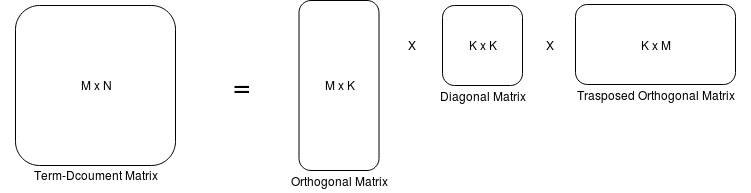
\includegraphics[width=15cm,height=20cm,keepaspectratio]{images/LSIk.png}
	\caption{Reduction phase}
	\label{fig:LSIk}
\end{figure}

Figure \ref{fig:LSIk} depicts the low rank reduction phase and is interesting to graphically see what does it mean. The new matrix is the product of the other three, but reducted, this is a very relevant issue. If the singular values in $S_{mn}$ are ordered by size, the first k largest may be kept and the remaining smaller ones set to zero. The product of the resulting matrices is a matrix $X$ which is only approximately equal to $A_{mm}$ , and is of rank k . It can be shown that the new matrix $X$ is the matrix of rank k which is closest in the least squares sense to $A_{mm}$ .
The amount of dimension reduction, i.e., the choice of k , is critical to our work. Ideally, we want a value of k that is large enough to fit all the real structure in the data, but small enough so that we do not also fit the sampling error or unimportant details. The proper way to make such choices is an open issue in the factor analytic literature. In practice, we currently use an operational criterion - a value of k which yields good retrieval performance.\\ In our work we decided a \emph{k value =} $\frac{repository}{2}$

\clearpage
%%%%%%%%%%%%%%%%%%%%%%%%%%%%%%%%%%%%%%%%%%%%%%%%%%%%%%%%%%  
\subsection{Knowledge-Based}
Knowledge-Based Similarity aims to identify the degree of similarity between words using informations derived from semantic networks.
Knowledge-based similarity measures can be divided roughly into two groups: measures of semantic similarity and measures of semantic relatedness.By semantic similarity we mean concepts that are related each other on the basis of their likeness.
Semantic relatedness, on the other hand, is a more general notion of relatedness, not specifically tied to the shape or form of the concept. Semantic similarity is a metric defined over a set of documents or terms, where the idea of distance between them is based on the likeness of their meaning or semantic content as opposed to similarity which can be estimated regarding their syntactical representation (e.g. their string format).
An example of relatedness is the Lask algorithm which identify senses of words in context using definition overlap. To clarify let's take a look an example in \cite{Resnik}.
Using the Oxford Advanced Learner's Dictionary, it finds that word \emph{pine} has two senses:
\begin{itemize}
	\item{Sense 1: kind of \textbf{evergreen tree} with needle-shaped leaves}
	\item{Sense 2: waste away through sorrow ir illness.}
\end{itemize}

The word \emph{cone} has three senses:
\begin{itemize}
	\item{Sense 1: solid body which narrows to a point}
	\item{Sense 2: something of this shape whether solid or hollow}
	\item{Sense 3: fruit of certain \textbf{evergreen tree}}
\end{itemize}

Each of the two senses of the word \emph{pine} is compared with each of the three senses of the \emph{cone} and it is found that the words \emph{evergreen tree} occurs in one sense each of the two words. These two senses are then declared to be the most appropriate senses when words \emph{pine} and \emph{cone} are used togheter.

Concerning the similarity an example could be Resnik(1995) which uses the information content of concepts, computed from their frequency of occurrence in a large corpus, to determine the semantic relatedness of word senses\cite{Resnik}.
Another example is Jian \& Conrath \cite{Jian}s It combines a lexical taxonomy structure with corpus statistical information so that the semantic distance between nodes in the semantic space constructed by the taxonomy can be better quantified with the computational evidence derived from a distributional analysis of corpus data. Specifically, the proposed measure is a combined approach that inherits the edge-based approach of the edge counting scheme, which is then enhanced by the node-based approach of the information content calculation.

		\clearpage

		\section{The Approaches}
		\label{sec:Approaches}
		%%%%%%%%%%%%%%%%%%%%%%%%%%%%%%%%%%%%%%%%%%%%%%%%%%%%%%%%%%

\subsection{MUDABlue}\label{sec:mudablue}

The first procedure analysed was MUDABlue, unfortunately none implentation was available on the web, so i reimplemented it from scratch. The MUDABlue method is an automatc categorizaton method or a large collecton of software systems. MUDABlue method does not only categorize sooware systemsd but also determines categories rom the sooware systems collecton automatcally. MUDABlue has three major aspects: 1) it relies on no other information than the source code, 2) it determines category sets automatically, and 3) it allows a software system to be a member of multiple categories. Since we were interested only in the evaluation of the similarity we discarded the phases related to clusterization and categorization.

\subsection{The Approach}

The MUDABlue approach can be briefly summarized in 7 steps, as the following image depicts:

\begin{figure}[H]
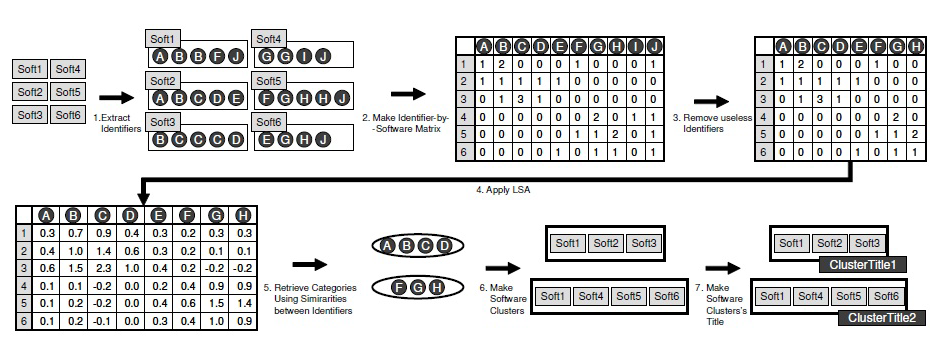
\includegraphics[width=15cm,height=20cm,keepaspectratio]{images/Mudablue1.png}
\centering
\caption{MUDABlue phases.}
\end{figure}

\subsubsection{Exctract Identifiers}
With identifier we are talking about relevant strings that can allow to characterize a document. In this phase each repository is scanned in order to find the target files, and for each of them the identifiers are exctracted, avoiding adding useless items such as comments. The dataset was a 41C projects gathered from SourceForge.

\subsubsection{Create identifier-by-software matrix}
As stated before, the main item to work with is the term-document matrix, in this case we count how many times each term appears in each file for all the projects. The result is matrix \textbf{m x n} with m terms and n projects.

\subsubsection{Remove useless identifiers}
From the matrix we remove all the useless terms, that is all the terms that apperas in just one repository, considered a specific terms, and all the terms that appears in more than 50\% of the repositories, considered as general terms.

\subsubsection{Apply the LSA}
Once the matrix is ready con be worked, the SVD procedure is applied and then the LSI. As explained before [NOTE] the SVD procedure decompose the original matrix in 3 other matrices. When we multiply back these matrices we use a rank reducted version of the S matrix in order to generete the final one. The authors didn't provide us any details about their final rank value, so we tested many values and eventually selected one.

\subsubsection{Apply the Cosine Similarity}
By using the cosine similarity method, we compare each repository vector with all the others and eventually getting an \textbf{n x n} matrix, in which is expressed the similarity of all the repository couple, with a value [0.0-1.0].

\subsubsection{Categorization}
The point 6 and 7 are not covered because not related to our work.
\clearpage



%%%%%%%%%%%%%%%%%%%%%%%%%%%%%%%%%%%%%%%%%%%%%%%%%%%%%%%%%%

\subsection{CLAN:  Closely reLated ApplicatioNs}\label{sec:clan}

\textit{CLAN} \cite{McMillan:2012:DSS:2337223.2337267} is an approach for automatically detecting similar Java applications by exploiting the semantic layers corresponding to packages class hierarchies. \textit{CLAN} works based on the document framework for computing similarity, semantic anchors, e.g. those that define the documents' semantic features. Semantic anchors and dependencies help obtain a more precise value for similarity computation between documents. The assumption is that if two applications have API calls implementing requirements described by the same abstraction, then the two applications are more similar than those that do not have common API calls. The approach uses API calls as semantic anchors to compute application similarity since API calls contain precisely defined semantics. The similarity between applications is computed by matching the semantics already expressed in the API calls.

\subsection{The Approach}

The process consist of 12 steps here graphically reported.

\begin{figure}[H]
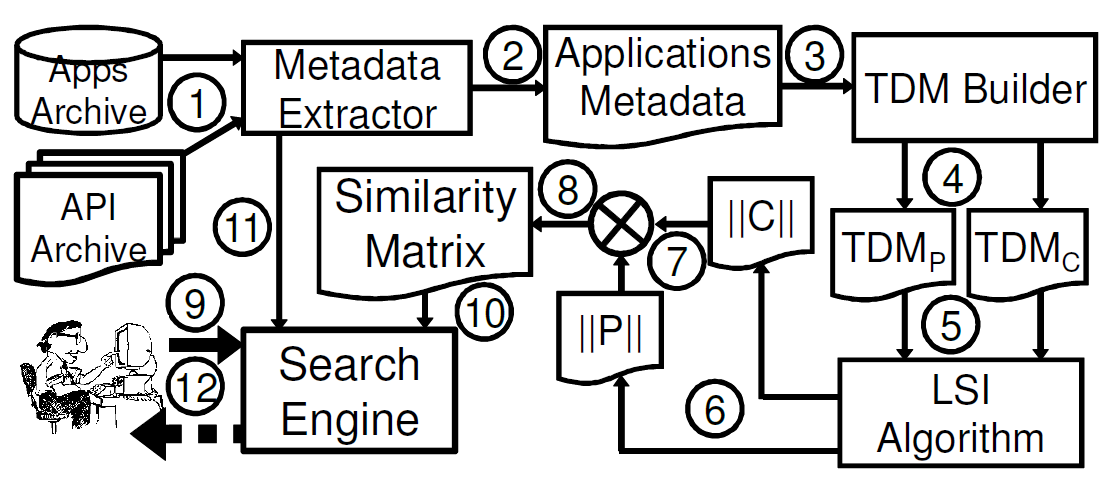
\includegraphics[width=15cm,height=20cm,keepaspectratio]{images/Clan.png}
\centering
\caption{CLAN phases.}
\end{figure}

\subsubsection{1 - 3: Terms Extraction}
Steps from 1 to 3 can be merged together since are related to extraction of terms from the repositories.
As stated before, an important concept is that terms extracted are only API calls, this means that all other things present in a piece of code are discarded, for example all the variables or the function declaration and invocation. Furthermore these API calls belong only to the JDK, in such a way also the calls to any other external library are discarded. This idea is also applied in the extraction of the import declaration, focus only on the JDK packages import.
The result of this process will be an ordered set of data, representing the occurrencies of any Package;Class for all the projects.

\subsubsection{4: TDMs Creation}
Once the dataset as been created, is reorganized in TDMs. Here two different matrices are created, one for the Classes and one for the Packages. Class-level and package-level similarities are different since applications are often more similar on the package level than on the class level because there are fewer packages than classes in the JDK. Therefore, there is the higher probability that two applications may have API calls that are located in the same package but not in the same class.

\subsubsection{5: LSI Procedure}

\subsubsection{6: Apply the Cosine Similarity}

\subsubsection{7: Sum of the matrices}
The 2 matrices are summed, but before are multplied by a certain value. Since the values for the entries in the 2 matrices are between 0.0 and 1.0 a simple sum could result in a value over 1.0, by this multiplication these values are reducted in order to be summed togheter but still maintaining the logical meaning. The authors chosen 0.5, also we, since is a good value to equal distribute the weight of the packages and method calls.The sum of this value is 1.0, and can span from 0.1 to 0.9 for each matrix, is clear that more is high on a matrix, more is important the values that we are considering from such matrix.

\subsubsection{8: Final similarity matrix}
\clearpage


%%%%%%%%%%%%%%%%%%%%%%%%%%%%%%%%%%%%%%%%%%%%%%%%%%%%%%%%%%  

\subsubsection{RepoPal: Exploiting Metadata to Detect Similar GitHub Repositories}\label{sec:repopal}

In contrast to many previous studies that are generally based on source code \cite{10.1109/APSEC.2004.69},\cite{Liu:2006:GDS:1150402.1150522},\cite{McMillan:2012:DSS:2337223.2337267}, \textit{RepoPal}  \cite{10.1109/SANER.2017.7884605} is a high-level similarity metric and takes only repositories metadata as its input. With this approach, two GitHub repositories are considered to be similar if:

\begin{itemize}
	\item[i)] They contain similar readme files;
	\item[ii)] They are starred by users of similar interests;
	\item[iii)] They are starred together by the same users within a short period of time. 
\end{itemize}

Thus, the similarities between GitHub repositories are computed by using three inputs: readme file, stars and the time gap that a user stars two repositories. Considering two repositories $ r_{i} $ and $ r_{j} $, the following notations are defined: 

\begin{itemize}
	\item $ f_{i} $ and $ f_{j} $ are the readme files with $ t $ being the set of terms in the files; 
	\item $ U(r_{i}) $ and $ U(r_{j}) $ are the set of users who starred $ r_{i} $ and $ r_{j} $, respectively; 
	\item $ R(u_{k}) $ is the set of repositories that user $ u_{k} $ already starred.  
\end{itemize}

There are three similarity indices as follows:

\paragraph{Readme-based similarity} 

The similarity between two readme files is calculated as the cosine similarity between their feature vectors $\vec{f_{i}}$ and $\vec{f_{j}}$: 

\begin{equation}
sim_{f}(r_{i},r_{j})=CosineSim(\vec{f_{i}},\vec{f_{j}})
\end{equation}
		\clearpage

		\section{Evaluation}
		\label{src:Evaluation}
		%\section{Overview}
%As stated before we opted for \emph{MUDABLUE} and \emph{CLAN}. The rationale behind the selection of these approaches is that they are well-established algorithms. 





In this section we discuss the process that has been conceived and applied to evaluate the performance the four approaches introduced in Chapter~\ref{sec:Implementation}. To this end, the evaluation process that has been applied is shown in Figure~\ref{fig:EvaluationProcess} and consists of activities and artifacts that are going to be explained later on this chapter. In particular, a set of Java projects (Section~\ref{sec:Dataset}) has been crawled to feed as input for the computation by all approaches, \ie \MUDABlue, \CLAN, \RepoPal, and \CrossSim. Afterwards, a set of projects is selected as queries to compute similarities against all the remaining OSS projects (Section~\ref{sec:Queries}). Once the scores have been computed, for each similarity tool, some of the top similar projects are chosen, and mixed to be evaluated by humans (Section~\ref{sec:UserStudy}). The results are then evaluated using various quality metrics (Section~\ref{sec:Metrics}).


\begin{figure}[h!]
	\centering
	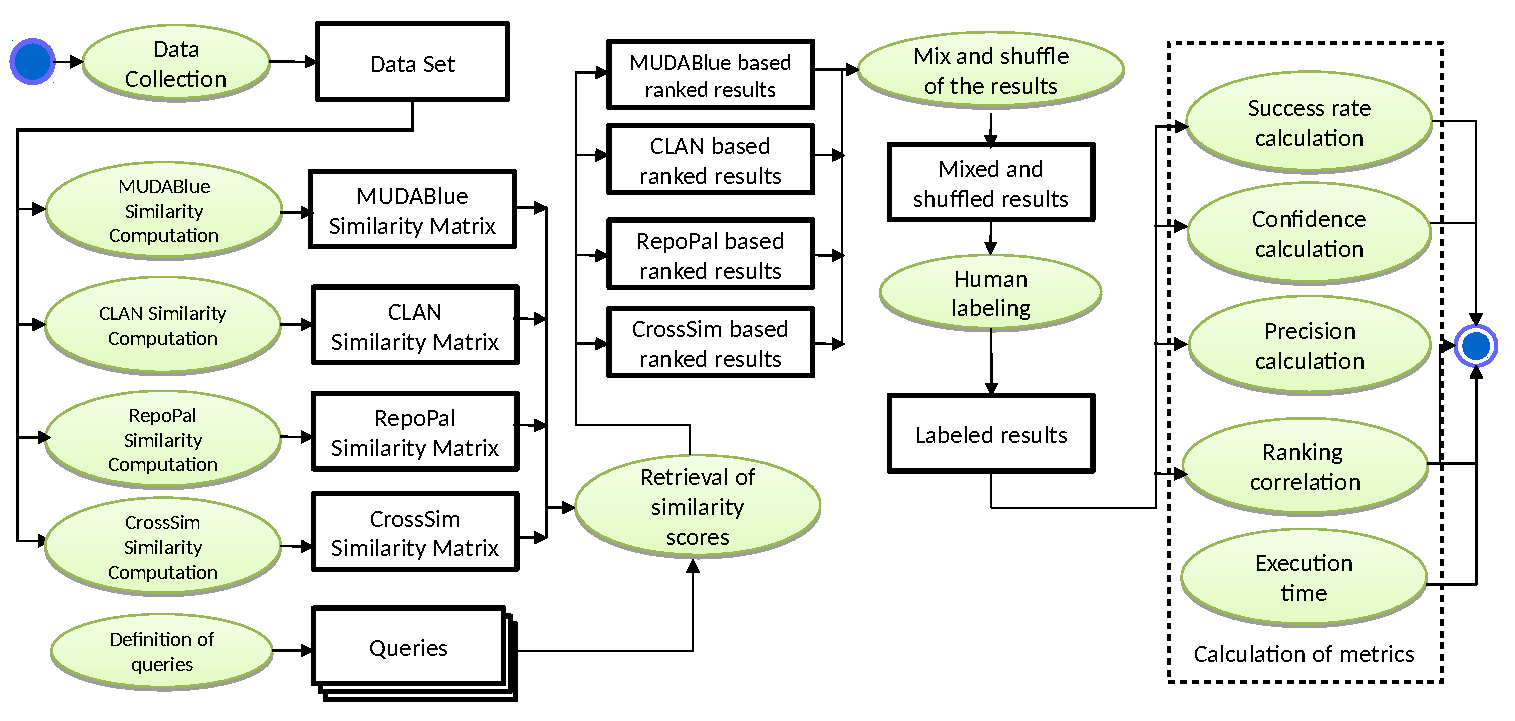
\includegraphics[width=0.99\linewidth]{images/EvaluationProcess}
	\caption{Evaluation process}
	\label{fig:EvaluationProcess}
\end{figure}








\section{Dataset} \label{sec:Dataset}

To serve as input for the evaluation, it is necessary to populate a dataset that meets the requirements by all four approaches. By MUDABlue and CLAN, there are no specific requirements since both metrics rely solely on source code to function. However, for CrossSim, we consider only projects that satisfy certain criteria. In particular, we collected projects that meet the following requirements:

\begin{itemize}
	\item Being GitHub Java projects; 
	\item Providing the specification of their dependencies by means of \code{code.xml} or \code{gradle} files;
	\item Including at least $9$ dependencies. A project with no or little information about dependencies may adversely affect the performance of \CrossSim; 
	\item Having the \code{README.md} file available.
\end{itemize}

Furthermore, we realized that the final outcomes of a similarity algorithm are to be validated by human beings, and in case the projects are irrelevant by their very nature, the perception given by human evaluators would also be \emph{dissimilar} in the end. This is valueless for the evaluation of similarity. Thus, to facilitate the analysis, instead of crawling projects in a random manner, we first observed projects in some specific categories (e.g. PDF processors, JSON parsers, Object Relational Mapping projects, and Spring MVC related tools). Once a certain number of projects for each category had been obtained, we also started collecting randomly to get projects from various categories.

Using the GitHub API\footnote{GitHub API: \url{https://developer.github.com/v3/}}, we crawled projects to provide input for the evaluation. Though the number of projects that fulfill the requirements of a single approach, i.e. either RepoPal or CrossSim, is high, the number of projects that meet the requirements of both approaches is considerably lower. For example, a project contains both \code{pom.xml} and \code{README.md}, albeit having only $5$ dependencies, does not meet the constraints and must be discarded. The crawling is time consuming as for each project, at least $6$ queries must be sent to get the relevant data. GitHub already sets a rate limit for an ordinary account\footnote{GitHub Rate Limit: \url{https://developer.github.com/v3/rate_limit/}}, with a total number of $5,000$ API calls per hour being allowed. And for the search operation, the rate is limited to $30$ queries per minute. Due to these reasons, we ended up getting a dataset of $580$ projects that are eligible for the evaluation. The dataset we collected and the CrossSim tool are already published online for public usage \cite{CROSSSIM-DATA}.

%\subsection{Data collection} \label{sec:DataCollection}
%In addition, to facilitate the evaluation of similarity and clustering techniques, instead of crawling projects in a random manner, we first observed projects in some specific categories. We suppose that the evaluation might lead to a cumbersome process if we consider arbitrary projects which are generally not related. The final outcomes of a similarity algorithm need to be validated by human beings, and given that the projects are irrelevant by their very nature, the perception given by human evaluators would also be \emph{dissimilar} in the end, and this is valueless for the evaluation of similarity. 

\begin{table}[h!]
%	\small
	\centering
	\begin{tabular}{|p{0.80cm}|p{6.00cm}|p{2.80cm}|}  \hline
		{\bf No.} & {\bf Name} & {\bf \# of Projects} \\  \hline
		1 & SPARQL, RDF, Jena Apache & 21 \\  \hline
		2 & PDF Processor & 8  \\  \hline
		3 & Selenium Web Test & 26  \\  \hline
		4 & ORM & 13  \\  \hline
		5 & Spring MVC & 51  \\  \hline
		6 & Music Player & 25  \\  \hline
		7 & Boilerplate & 38  \\  \hline
		8 & Elastic Search & 55  \\  \hline
		9 & Hadoop, MapReduce & 52  \\  \hline
		10 & JSON & 20  \\  \hline
		11 & Miscellaneous Categories & 271  \\  \hline
	\end{tabular}
	\caption[List of software categories]{List of software categories}
	\label{tab:Categories}
\end{table}


Further than collecting projects for each category, we also started collecting random projects. These projects serve as a means to test the stability of the algorithms. If the algorithms work well, they will not perceive newly added random projects as similar to projects of some other specific categories. To this end, the categories and their corresponding cardinality to be studied in our evaluation are listed in Table \ref{tab:Categories}. This is an approximate classification since a project might belong to more than one category.

As can be seen in Table \ref{tab:Categories}, among $580$ considered projects, $309$ of them belong to some specific categories, such as \emph{SPARQL, RDF, Jena Apache}, \emph{Selenium Test}, \emph{Elastic Search}, \emph{Spring MVC}, etc. The other $271$ projects being selected randomly belong to \emph{Miscellaneous Categories}. These categories disperse in several domains and sometimes it happens that there is only one project in a category. For the sake of clarity, we do not introduce the list of the categories in this thesis.

%The random projects are used as a means to.
%From the dataset, a graph is built using the relationships in Section~\ref{sec:GraphRepresentation}. %There, nodes are either users, dependencies or projects and each is encoded using a unique number across the whole graph. Edges represent the corresponding relationships between users and projects or between dependencies and projects. 
%\paragraph{\textbf{Application of RepoPal and CrossSim}}
%\noindent\emph{\textbf{Application of RepoPal and CrossSim}}



\section{Query definition} \label{sec:Queries}

Among $580$ projects in the dataset, $50$ have been selected as queries and they are listed in Table \ref{tab:Queries}. To aim for variety, the queries have been chosen to cover different categories, e.g.: SPARQL and RDF, Selenium Test, Elastic Search, Spring MVC, Hadoop, Music Player.

\begin{table}[!h]
	\footnotesize
	\centering
	\begin{tabular}{|p{0.80cm}|p{6.0cm}|p{0.80cm}|p{6.0cm}|}  \hline
		{\bf No.} & {\bf Name} & {\bf No.} & {\bf Name} \\  \hline
		1 & \href{https://github.com/neo4j-contrib/sparql-plugin}{neo4j-contrib/sparql-plugin}  & 26 & \href{https://github.com/mariamhakobyan/elasticsearch-river-kafka}{mariamhakobyan/elasticsearch-river-kafka} \\ \hline
		2 & \href{https://github.com/AskNowQA/AutoSPARQL}{AskNowQA/AutoSPARQL} & 27 & \href{https://github.com/OpenTSDB/opentsdb-elasticsearch}{OpenTSDB/opentsdb-elasticsearch} \\ \hline
		3 & \href{https://github.com/AKSW/Sparqlify}{AKSW/Sparqlify} & 28 & \href{https://github.com/codelibs/elasticsearch-cluster-runner}{codelibs/elasticsearch-cluster-runner} \\ \hline
		4 & \href{https://github.com/AKSW/SPARQL2NL}{AKSW/SPARQL2NL} & 29 & \href{https://github.com/opendatasoft/elasticsearch-plugin-geoshape}{opendatasoft/elasticsearch-plugin-geoshape} \\ \hline 
		5 & \href{https://github.com/pyvandenbussche/sparqles}{pyvandenbussche/sparqles} & 30 &  \href{https://github.com/huangchen007/elasticsearch-rest-command}{huangchen007/elasticsearch-rest-command} \\ \hline
		6 & \href{https://github.com/sayems/java.webdriver}{sayems/java.webdriver} & 31 & \href{https://github.com/pitchpoint-solutions/sfs}{pitchpoint-solutions/sfs} \\ \hline
		7 & \href{https://github.com/xebia/Xebium}{xebia/Xebium} & 32 & \href{https://github.com/javanna/elasticsearch-river-solr}{javanna/elasticsearch-river-solr} \\ \hline
		8 & \href{https://github.com/webdriverextensions/webdriverextensions}{webdriverextensions/webdriverextensions} & 33 & \href{https://github.com/mesos/hadoop}{mesos/hadoop} \\ \hline
		9 & \href{https://github.com/testIT-WebTester/webtester-core}{testIT-WebTester/webtester-core} & 34 & \href{https://github.com/pentaho/big-data-plugin}{pentaho/big-data-plugin} \\ \hline
		10 & \href{https://github.com/seleniumQuery/seleniumQuery}{seleniumQuery/seleniumQuery} & 35 & \href{https://github.com/asakusafw/asakusafw}{asakusafw/asakusafw} \\ \hline
		11 & \href{https://github.com/bonigarcia/webdrivermanager}{bonigarcia/webdrivermanager} & 36 & \href{https://github.com/klarna/HiveRunner}{klarna/HiveRunner} \\ \hline
		12 & \href{https://github.com/selenium-cucumber/selenium-cucumber-java}{selenium-cucumber/selenium-cucumber-java} & 37 &
		\href{https://github.com/sonalgoyal/hiho}{sonalgoyal/hiho} \\ \hline
		13 & \href{https://github.com/conductor-framework/conductor}{conductor-framework/conductor} & 38 & \href{https://github.com/pranab/beymani}{pranab/beymani} \\ \hline
		14 & \href{https://github.com/caelum/vraptor}{caelum/vraptor} & 39 & \href{https://github.com/lintool/Ivory}{lintool/Ivory} \\ \hline 
		15 & \href{https://github.com/caelum/vraptor4}{caelum/vraptor4} & 40 & \href{https://github.com/GoogleCloudPlatform/bigdata-interop}{GoogleCloudPlatform/bigdata-interop} \\ \hline
		16 & \href{https://github.com/KEN-LJQ/WMS}{KEN-LJQ/WMS} & 41 & \href{https://github.com/Conductor/kangaroo}{Conductor/kangaroo} \\ \hline
		17 & \href{https://github.com/white-cat/jeeweb}{white-cat/jeeweb} & 42 & \href{https://github.com/datasalt/pangool}{datasalt/pangool} \\ \hline
		18 & \href{https://github.com/livrospringmvc/lojacasadocodigo}{livrospringmvc/lojacasadocodigo} & 43 & \href{https://github.com/laserson/avro2parquet}{laserson/avro2parquet} \\ \hline
		19 & \href{https://github.com/spring-projects/spring-mvc-showcase}{spring-projects/spring-mvc-showcase} & 44 & \href{https://github.com/Knewton/KassandraMRHelper}{Knewton/KassandraMRHelper} \\ \hline
		20 & \href{https://github.com/sonian/elasticsearch-jetty}{sonian/elasticsearch-jetty} & 45 & \href{https://github.com/blackberry/KaBoom}{blackberry/KaBoom} \\ \hline
		21 & \href{https://github.com/dadoonet/spring-elasticsearch}{dadoonet/spring-elasticsearch} & 46 & \href{https://github.com/jt6211/hadoop-dns-mining}{jt6211/hadoop-dns-mining} \\ \hline
		22 & \href{https://github.com/elastic/elasticsearch-metrics-reporter-java}{elastic/elasticsearch-metrics-reporter-java} & 47 & \href{https://github.com/psaravan/JamsMusicPlayer}{psaravan/JamsMusicPlayer} \\ \hline
		23 & \href{https://github.com/elastic/elasticsearch-support-diagnostics}{elastic/elasticsearch-support-diagnostics} & 48 & \href{https://github.com/TheAndroidMaster/Pasta-Music}{TheAndroidMaster/Pasta-Music} \\ \hline
		24 & \href{https://github.com/SpringDataElasticsearchDevs/spring-data-elasticsearch}{SpringDataElasticsearchDevs/spring-data-elasticsearch} & 49 & \href{https://github.com/SubstanceMobile/GEM}{SubstanceMobile/GEM} \\ \hline
		25 & \href{https://github.com/javanna/elasticshell}{javanna/elasticshell} & 50 & \href{https://github.com/markzhai/LyricHere}{markzhai/LyricHere} \\ \hline
		
	\end{tabular}
	\caption[List of queries]{List of queries for evaluation}
	\label{tab:Queries}
\end{table}


% Three postgraduate students participated in the user study with two of them being
% Given a query, a user study is performed Evaluators are asked to label the similarity for each pair of projects (i.e., $<$\textit{query, retrieved project}$>$) with regards to their application domains and functionalities using the scales listed in Table \ref{tab:Scales}. 

%\section{Retrieval of similarity scores}
%
%Our evaluation has been conducted in line with some other existing studies \cite{Lo:2012:DSA:2473496.2473616},\cite{McMillan:2012:DSS:2337223.2337267},\cite{10.1109/SANER.2017.7884605}. For each query, similarity is computed against all the remaining projects in the dataset using \CrossSim. From the retrieved projects, only top $5$ are selected for evaluation. For each query, similarity is also computed using $RepoPal$ and other similarity metrics in Section \ref{sec:Baselines} to get the top-$5$ most similar retrieved projects.
%


\section{User Study} \label{sec:UserStudy}

%We involved a group of $15$ people software developers who have at least 5 years of experience in the user study. To get information about the participants related to their programming experience, we sent them a questionnaire similar to the one presented in \cite{McMillan:2012:DSS:2337223.2337267}. According to the survey, we found out that most developers use StackOverflow to search for code. %\footnote{\url{http://www.cs.wm.edu/semeru/clan/CaseStudyMaterials.zip}}. 
%Three postgraduate students in Computer Science who possess a good programming experience were invited to 
%In order to have a fair evaluation, for each query we mix and shuffle the top-$5$ results generated from the computation by all similarity metrics in a single file and present them to the evaluators. This mimics a \emph{taste test}\footnote{Taste Test: Is Bottled Better? \url{http://www.scwa.ca.gov/files/docs/outreach/water-ed/activities/Taste\%20Test.pdf}} where users are asked to evaluate a product, e.g. food or drink, without having a priori knowledge about what is being addressed. This helps eliminate any bias or prejudice against a specific similarity metric. Bias can be any preference given to a pre-known metric and any type of bias would considerably undermine the evaluation outcomes.%deteriorate
%In particular, given a query, a developer is asked to evaluate the similarity between the query and the corresponding retrieved projects. 


We performed a user study following the descriptions in \cite{Lo:2012:DSA:2473496.2473616},\cite{McMillan:2012:DSS:2337223.2337267},\cite{10.1109/SANER.2017.7884605} to evaluate the similarity between query projects and their corresponding retrieved projects. A group of $15$ software developers who have at least 5 years of experience took part in the experiments. In order to have a fair evaluation, for each query we mixed and shuffled the top-$5$ results generated from the computation by all similarity metrics in a single file and present them to the evaluators. This mimics a \emph{taste test} where users are asked to evaluate a product, \eg food or drink, without having a priori knowledge about what is being addressed \cite{Ghose2001},\cite{doi:10.1108/13522750810879048}. This aims at eliminating any bias or prejudice against a specific similarity metric. The participants are asked to label the similarity for each pair of projects (\ie $<$\textit{query, retrieved project}$>$) with regards to their application domains and functionalities using the scales listed in Table \ref{tab:Scales} \cite{McMillan:2012:DSS:2337223.2337267}. For example, an OSS project $p_{1}$ that performs the sending of files across a TCP/IP network is somehow similar to an OSS project $p_{2}$ that exchanges text messages between two users, \ie $Score(p_{1},p_{2})=3$. However an OSS project $p_{3}$ with the functionalities of a pure text editor is dissimilar to both $p_{1}$ and $p_{2}$, \ie $Score(p_{1},p_{2})=Score(p_{1},p_{3})=1$. Given a query, a retrieved project is considered as a \emph{false positive} if its similarity to the query is labeled as \code{Dissimilar} ($1$) or \code{Neutral} ($2$). In contrast, \emph{true positives} are those retrieved projects that have a score of $3$ or $4$, \ie \code{Similar} of \code{Highly similar}. A good similarity metric should produce as much true positives as possible.

\begin{table*}[h!]
	\centering
	\begin{tabular}{|p{3.0cm}|p{8.0cm}|p{1.0cm}|}  \hline
		{\bf Scale} & {\bf Description} & {\bf Score} \\  \hline
		Dissimilar & The functionalities of the retrieved project are completely different from those of the query project & 1 \\ \hline
		Neutral & The query and the retrieved projects share a few functionalities in common & 2 \\ \hline
		Similar & The two projects share a large number of tasks and functionalities in common & 3 \\ \hline
		Highly similar & The two projects share many tasks and functionalities in common and can be considered the same & 4 \\ \hline
	\end{tabular}
	\caption[The similarity scales]{Similarity scales}
	\label{tab:Scales}
\end{table*}


The participants are asked to label the similarity for each pair of projects (i.e., $<$\textit{query, retrieved project}$>$) with regards to their application domains and functionalities using the scales listed in Table \ref{tab:Scales}. For example, an OSS project $p_{1}$ that performs the sending of files across a TCP/IP network is somehow similar to an OSS project $p_{2}$ that exchanges text messages between two users, i.e. $Score(p_{1},p_{2})=3$. However an OSS project $p_{3}$ with the functionalities of a pure text editor is dissimilar to both $p_{1}$ and $p_{2}$, i.e. $Score(p_{1},p_{2})=Score(p_{1},p_{3})=1$. Given a query, a retrieved project is considered as a \emph{false positive} if its similarity to the query is labelled as Dissimilar ($1$) or Neutral ($2$). In contrast, \emph{true positives} are those retrieved projects that have a score of $3$ or $4$, i.e. Similar of Highly similar. A good similarity metric should produce as much true positives as possible.


\section{Evaluation Metrics} \label{sec:Metrics}

To evaluate the outcomes of the algorithms with respect to the user study, the following metrics have been considered as typically done in related work \cite{Lo:2012:DSA:2473496.2473616,McMillan:2012:DSS:2337223.2337267,10.1109/SANER.2017.7884605}:

\begin{itemize}
	\item \textit{Success rate}: if at least one of the top-5 retrieved projects is labelled \emph{Similar} or \emph{Highly similar}, the query is considered to be successful. {\em Success rate} is the ratio of successful queries to the total number of queries;
	\item \textit{Confidence}: Given a pair of $<$\textit{query, retrieved project}$>$ the confidence of an evaluator is the score she assigns to the similarity between the projects;
	\item \textit{Precision}: The precision for each query is the proportion of projects in the top-5 list that are labelled as \emph{Similar} or \emph{Highly similar} by humans. 
\end{itemize}

Further than the previous metrics, we introduce an additional one to measure the ranking produced by the similarity tools. For a query, a similarity tool is deemed to be good if all top-5 retrieved projects are relevant. In case there are false positives, i.e. those that are labeled \emph{Dissimilar} and \emph{Neutral}, it is expected that these will be ranked lower than the true positives. In case an irrelevant project has a higher rank than that of a relevant project, we suppose that the similarity tool is generating an improper recommendation. The \emph{Ranking} metric presented below is a means to evaluate whether a similarity metric produces properly ranked recommendations. 





\section{Results} \label{sec:Results}

To study the performance of the metrics in detecting similar projects for the set of queries, the following research questions are considered:

\newcommand{\rqfirst}{RQ$_1$: Which similarity metric yields a better performance in terms of Success rate, and Precision?}\textit{\textbf{\rqfirst}} 

By this question, we study the performance of different approaches.

\begin{figure}[!h]
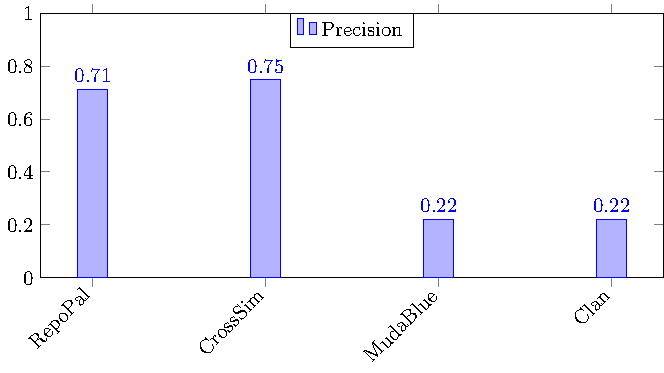
\includegraphics[width=10cm,height=15cm,keepaspectratio]{images/Precision.pdf}
\centering
\caption{Precision Comparison}
\label{fig:PrecisionC}
\end{figure}

Experimental results suggests that CrossSim approach overperforms all the other approaches, in particular Clan and MudaBlue.
Repopal got a good score, this means that is still a valid choice for similarity in the OSS environment.
The precision,as the figure~\ref{fig:PrecisionC} depicts, shows that CrossSim and Repopal got a score \emph{greater than 70\%}.
Clan and MudaBlue instead, reported a very low score, \emph{about 20\%}, on 10 queries evaluted, just 2 got a score \emph{$\geq3$}.

\begin{figure}[!h]
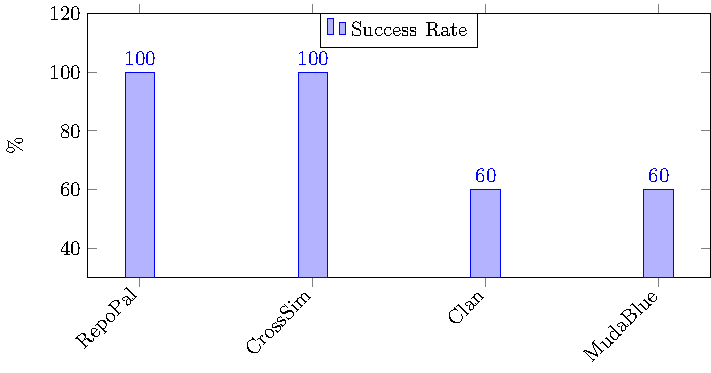
\includegraphics[width=10cm,height=15cm,keepaspectratio]{images/SuccessRate.pdf}
\centering
\caption{Success Rate Comparison}
\label{fig:SuccessC}
\end{figure}

Concerning the success rate, the results of CrossSim and Repopal are quite impressive, about \emph{100\%} of queries got score high, the situation is lower for Clan and MudaBlue that achieved just the \emph{60\%} of the queries. In order to calculate this values, we counted for each query how many votes were \emph{$\geq3$} divided then by 25, which is the number of queries.


\begin{figure}[!h]
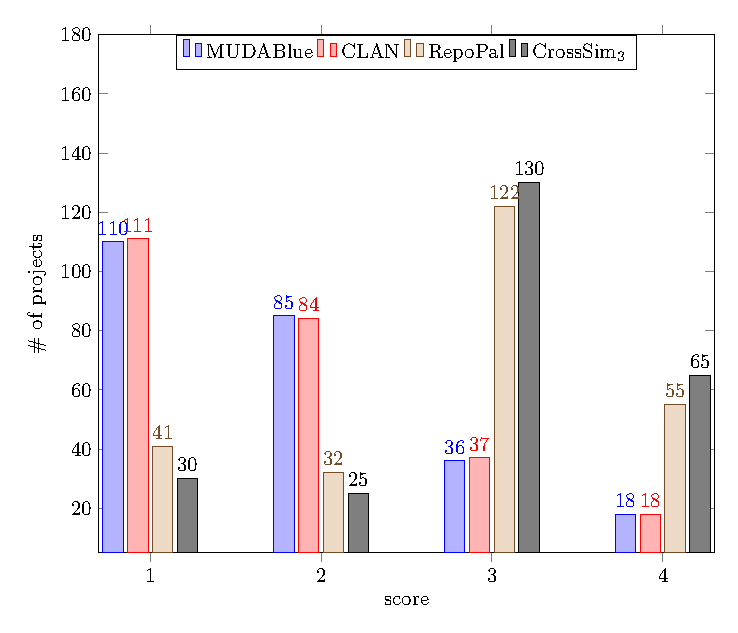
\includegraphics[width=10cm,height=15cm,keepaspectratio]{images/Confidence.pdf}
\centering
\caption{Confidence Comparison}
\label{fig:ConfidenceC}
\end{figure}

The confidence confirms what stated so far, the mojority of the votes for MudaBlue and Clan are between 1 and 2,that is, users evaluated as dissimilar most of the projects. For CrossSim the result is quite more nice, with 130 rank 3 votes and 60 rank 4 votes, so more than half results are good. Repopal also got a good evaluation, close to CrossSim but a bit lower.

\newcommand{\rqsecond}{RQ$_2$: Which similarity metric is more efficient?}\textit{\textbf{\rqsecond}} 

An important factor for a similarity metric is the ability to compute within an acceptable amount of time.

\begin{figure}[!h]
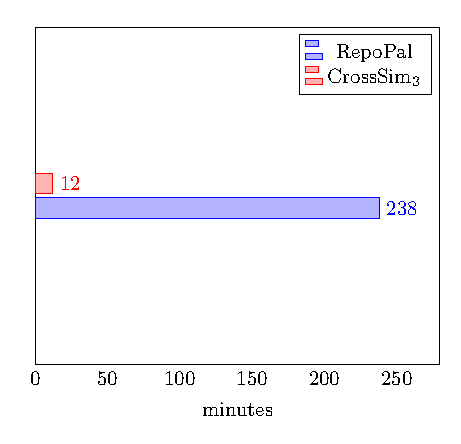
\includegraphics[width=8cm,height=13cm,keepaspectratio]{images/ExecutionTime.pdf}
\centering
\caption{Execution Time Comparison}
\label{fig:LabelC}
\end{figure}



\newcommand{\rqthird}{RQ$_3$: How does the graph structure affect the performance of \CrossSim?}\textit{\textbf{\rqthird}} 


When we consider \CrossSimA$_{1}$ in combination with \CrossSimA$_{2}$, the effect of the adoption of committers can be observed. \CrossSimA$_{1}$ gains a success rate of $100\%$, with a precision of $0.748$ and $63$ false positives. Whereas, the number of false positives by \CrossSimA$_{2}$ goes up to $76$, thereby worsening the overall performance considerably with $0.696$ being as the precision. The precision of \CrossSimA$_{2}$ is higher than those of $Readme$, $Dependency$, $Compound$, $Weighted$ $RepoPal$, but lower than those of $RepoPal$ and all of its \CrossSim counterparts. The performance degradation is further witnessed by considering \CrossSimA$_{3}$ and \CrossSimA$_{4}$ together. With respect to \CrossSimA$_{3}$, the number of false positives by \CrossSimA$_{4}$ increases by $5$ projects. We come to the conclusion that the inclusion of all developers who have committed updates at least once to a project in the graph is counterproductive as it adds a decline in precision. In this sense, we make an assumption that the deployment of a weighting scheme for developers may help counteract the degradation in performance. We consider the issue as our future work. 

Next, \CrossSimA$_{1}$ and \CrossSimA$_{3}$ are studied together to analyze the effect of the removal of the most frequent dependencies. \CrossSimA$_{3}$ outperforms \CrossSimA$_{1}$ as it gains a precision of $0.784$, the highest value among all, compared to $0.748$ by \CrossSimA$_{1}$. The removal of the most frequent dependencies helps also improve the performance of \CrossSimA$_{4}$ in comparison to \CrossSimA$_{2}$, which is a similar configuration, except that all dependencies are taken into account. Together, this implies that the elimination of too popular dependencies in the original graph is a profitable amendment. This is understandable once we get a deeper insight into the design of SimRank as already presented in Section \ref{sec:SimRank} and Figure \ref{fig:SimRank}. There, two projects are deemed to be similar if they share a same dependency, or in other words their corresponding nodes in the graph are pointed by a common node. However, with frequent dependencies as in Table \ref{tab:FrequentDeps} this characteristic may not hold anymore. Take as an example, two projects are pointed by a frequent dependency, e.g. \href{https://mvnrepository.com/artifact/junit/junit}{junit:junit} because they use JUnit\footnote{JUnit: Testing Framework for Java 8: \url{http://junit.org/junit5/}} for testing. And since testing is a common functionality of many software projects, it does not help contribute towards the characterization of a project and as a result, needs to be removed from similarity computation. 





\section{Threats to Validity}\label{sec:threatsValidity}

In this section, we investigate the threats that may affect the validity of the experiments as well as how we have tried to minimize them. In particular, we focus on the following threats to validity as discussed below. %internal and external 

\textit{\textbf{Internal validity}}  concerns any confounding factor that could influence our results.  We attempted to avoid any bias in the evaluation and assessment
phases: (\emph{i}) by involving three participants in the user study. In particular, the labeling results by one user were then double-checked by other two users to make sure that the outcomes were sound; (\emph{ii}) by completely automating the evaluation of the defined metrics without any manual intervention. Indeed, the implemented tools could be defective. To contrast and mitigate this threat, we have run several manual assessments and counter-checks.

\textit{\textbf{External validity}}  refers to the generalizability of obtained results and findings. Concerning the generalizability of our approach, we were able to consider a dataset of $580$ projects, due to the fact that the number of projects that meet the requirements of both RepoPal and CrossSim is low and thus required a prolonged crawling. During the data collection, we crawled both projects in some specific categories as well as random projects. The random projects served as a means to test the generalizability of our algorithm. If the algorithm works well, it will not perceive newly added random projects as similar to projects of the specific categories.

\textit{\textbf{Reliable validity}}  is related to the reproducibility of our experiments. To allow anyone to seamlessly replicate the evaluation, we made available the source code implementation of MUDABlue, CLAN, RepoPal, and CrossSim as also the dataset exploited in the paper in our GitHub repository \cite{CROSSSIM-DATA}.
		\clearpage

		\section{Conclusion}
		\label{src:Conclusion}
		The purpose of this work was providing a baseline result for the evaluation of a novel similarity calculator approach, CrossSim.
CrossSim is an approach developed by us inside the context of the CrossMiner project.

CROSSMINER\footnote{\url{https://www.crossminer.org}} is a research project funded by the EU Horizon 2020 Research and Innovation Programme, aiming at supporting the development of complex software systems by \textit{i)} enabling monitoring, in-depth analysis and evidence-based selection of open source components, and \textit{ii)} facilitating knowledge extraction from large OSS repositories \cite{10.1007/978-3-319-74730-9_33}. 

In order to provide such a baseline was mandatory to find some similar approach, we decided to use MudaBlue and Clan which are two close approaches, since there weren't any implementation available we re-implemented them from scratch. The contribute can be summarized as follows:

\begin{itemize}
	\item Study and Analysis of the problem. In this phase we have analyzed the similarity problem discovering that is well known problem studied in order to find a solution to some very interesting problems such as: (plagiarism detection, information retrieval,text classification, document clustering, topic detection and so on).In order to validate our novel approach we eventually decided to study in detail and implement two similarity calculator approaches: MudaBlue and Clan.
	\item Implementation. The implementation phase covered a lot of aspects. First of all was necessary analyzing the projects by parsing each \emph{.java} file and then summing up everything in a \emph{Term-Document matrix}. We applied then, the core of the apporaches, the \emph{Latent Semantic Analysis}, applying then the cosine similarity on the matrix we got the final matrix ready to be evaluated. The Ide was Eclipse and the language Java, with a lot of supporting library.
	\item Results Validation. At this stage we started the evaluation phase which consisted in a user study. We asked to a group of 10 people with experencie in Java delepoment, to rate a pull of queries provided by us. The results confirmed that CrossSim is a more precise method to calculate similarity with rispect to Clan and MudaBlue.
\end{itemize}

One of the most hard issue faced was related to the physical memory required to compute the Latent Semantic Analysis, for MudaBlue in particular we got something like \emph{700000} terms. This means that the required memory, only to manage the matrix was about 3Gb, this excluding all the memory used for other data structures and for the parsing. That's why we put a bound for the Eclipse virtual memory up to 8Gb and worked in two phase. During the first phase we collected all the terms by parsing everything and then, after an IDE restart, computing the LSA.

%%%%%Future Works%%%%%
Since the evualation was succesfully, in the sense that, results confirmed that CrossSim is a valuable similarity approach, the idea is to continue the development of the other features that still are missing (e.g. Code snippet suggestion, Api reccomandation).
		\clearpage

		\bibliographystyle{unsrt}
		\bibliography{ThesisDraft}

\end{document}
